\documentclass[a4paper]{usiinfbachelorproject}

\captionsetup{labelfont={bf}}
%%%%%%%%%%%%%%%%%%%%%%%%%%%% PACKAGES %%%%%%%%%%%%%%%%%%%%%%%%%%%%%
\usepackage{float}
\usepackage{amsmath}

%%% Main Body %%%

\author{Costanza Rodriguez Gavazzi}

\title{\textbf{How do children search?}}
\subtitle{A tool to support researchers in understanding how children search for information online}
\versiondate{\today}

\begin{committee}

\advisor[Universit\`a della Svizzera Italiana, Switzerland]{ }{Monica }{Landoni }

\coadvisor[Universit\`a della Svizzera Italiana, Switzerland]{ }{Diletta Micol}{Tobia}

\end{committee}

\abstract { Abstract goes here ...

Things to write: Context, Problem, Limitations in SOA, Contribution and Findings
\vspace{0.5em}

\textbf{Keywords}:
% You may include up to six keywords or phrases. Keywords should be separated with semicolons. 

}

\begin{document}
\maketitle
\tableofcontents
%\listoffigures\newpage

\newpage
%%%%%%%%%%%%%%%%%%%%%%%%%%%% INTRODUCTION %%%%%%%%%%%%%%%%%%%%%%%%%%%%%
\section{\textbf{Introduction}}



\newpage

%%%%%%%%%%%%%%%%%%%% BACKGROUND AND RELATED WORK %%%%%%%%%%%%%%%%%%%%%
\section{\textbf{Background and Related Work}}

The study of how children search for information online is a growing area that connects education, Information Retrieval (IR), and Human-Computer Interaction (HCI). The goal of this project was to develop a research tool that could collect interaction data from children using both traditional Search Engines and their Results Page (SERP), and Large Language Models (LLMs). Unlike other projects focused mainly on improving User Experience (UX) or User Interface (UI), this project was designed as a flexible platform to support various research questions on children's search behaviors. At the same time, the tool had to be fully functional and ready to use in real research scenarios, so an engaging and appropriate UI for younger users was still a key requirement.

\subsection{Foundation}

The starting point for this project was the bachelor's thesis by Savoia \cite{Savoia2025}. In her work, she proposed an interactive game designed to observe how children search for information. The interface was structured around a group of six islands, where each island represented a question framed with a specific emotional tone (positive, neutral, or negative). The children were allowed to choose how they wanted to answer the question, using a familiar web search interface or a chatbot-style LLM. Her work demonstrated that this narrative approach could encourage natural interactions and meaningful behavior from children.

Although her prototype successfully demonstrated the idea, it was not built with the core feature of data extrapolation, nor with reuse or extensibility in mind, but as a proof of concept. This project rebuilt the system from scratch to make it modular, maintainable, and suitable for future research experiments. Still, it kept the core idea of gameplay, the use of emotionally charged questions, and flexibility in tool choice to support various search strategies.

\subsection{Motivation}

A review of the literature highlighted the need for a research tool tailored to children's needs. Children are frequent users of Search Engines, especially in school settings, but often struggle to find relevant information efficiently \cite{Aliannejadi2021}. Most commercial tools like Google or Bing are designed for adults \cite{Aliannejadi2021, Landoni2021}, and there is no single search interface that fits all users, especially young people with different cognitive and emotional needs \cite{Landoni2021}.

In the IR research community, there is a clear call for child-friendly systems that are more suitable in educational contexts \cite{Landoni2020}. However, building such systems is challenging. Designing for children means taking into account their specific abilities: cognitive, technical, and emotional \cite{Chen2022}. In many cases, children say they want one thing, but their actual behavior shows something else. This is why relying only on interviews or post-task questionnaires can be misleading \cite{Aliannejadi2021}.

Besides, children are often left out of mainstream IR research and there is a lack of reliable data on how they really use search tools \cite{Savoia2025}. Researchers have highlighted the need for dedicated datasets, experimental tools, and evaluation methods designed for children \cite{Landoni2021c}.

Observing how children search and interact with systems, we can gather important insights that help improve the design of future tools \cite{Savoia2025}. These insights can also guide the development of features that help children, for example, by offering visual cues to highlight relevance or reduce confusion \cite{Landoni2021}. Data from child search behavior can also support many different research directions, including how emotions impact search performance, how children respond to positive or negative task formulation, or how task complexity affects engagement \cite{Landoni2020, Landoni2021c}. In particular, it is also interesting to consider how negative emotions are handled. Some research suggests that tracking negative user emotions could support better filtering, while others warn that hiding negative content could limit learning opportunities \cite{Landoni2020}.

A game-based tool, like the one built in this project, can collect structured data such as query logs, number of queries, time spent, and user clicks \cite{Aliannejadi2021}. It can also capture richer information about how children switch between tools or how many queries they need before answering. This kind of data would be difficult to gather with traditional observational methods or surveys, as children are reported to be unreliable sources when it comes to describing their own search behavior and preferences \cite{Aliannejadi2021}.

The strength of this approach comes from the benefits of game-based learning, which helps keep children engaged and motivated \cite{Alotaibi2024}. When children play a game, they tend to act more naturally and stay focused, making it easier to collect useful data on their behavior \cite{Alotaibi2024}. Compared to traditional learning environments, which can feel serious or stressful, games create a more relaxed space where children feel free to explore \cite{Alotaibi2024}.

By designing the tool as a digital game, we also benefit from interactive elements, storytelling, and visuals that make the experience fun.



\newpage

%%%%%%%%%%%%%%%%%%%%%%%%%%%% REQUIREMENTS %%%%%%%%%%%%%%%%%%%%%%%%%%%%%
\section{\textbf{Requirements}}

This project did not begin with a fixed list of specifications. Instead, requirements emerged iteratively through exploration of the research domain, analysis of related literature, and discussions with advisors. The work builds on Savoia's thesis \cite{Savoia2025}, which included an initial prototype of the game that was tested in a pilot session with children. From that experience, the feedback from the advisors and what we found in the literature,a new version of the game came to life, one that is more functional, scalable, and better suited to support different research questions in IR and HCI, while also being engaging and usable for children.

The main objective was to implement a fully functional and reusable prototype that could collect detailed data on how children use traditional SE and LLM, while also being engaging and usable for children. The project extends Savoia's prototype \cite{Savoia2025}, which demonstrated the potential of a game-based framework to study children's search behavior, but did not actually integrate the aspect of user data collection.
To structure the design, this dual purpose of the tool was fundamental: relevance for researchers aiming to study search behavior, and a pleasurable and engaging experience for children. From this core duality, the following questions guided the requirements definition process:
To structure the design, the following questions guided the requirement definition process.
\begin{itemize}
    \item What kind of data do researchers want to collect?
    \item Can a game-based interface be used to collect these data effectively?
    \item What kind of game design is both engaging and suitable for structured data collection?
    \item How can the tool be both usable for researchers and appealing to children?
    \item How can the system be modular, extensible, and maintainable for future research?
    \item How can it adapt to different experimental setups or research contexts?
\end{itemize}

These reflections acted as a guide to explore the literature, which then led to a concrete list of functional and non-functional requirements, discussed below.

\subsection{Data for Research Use}
Research has shown that a variety of data is needed to understand children's search behaviors.
This includes both quantitative metrics and qualitative observations. Although qualitative observations can offer several advantages in designing for children, this project's main focus was on quantitative metrics to enable the identification of patterns or relationships among behaviors. Analysis of these patterns can help researchers identify the potential roles of searchers among children \cite{Imazu2017}. Understanding these distinct roles that children play when searching is a key element in characterizing their behavior. Previous research \cite{Foss2012} defined seven roles for children searching in a home setting, based on qualitative data such as interviews and observations. More recent research \cite{Landoni2021c} aimed to understand the search roles of children, specifically in the classroom, and to see if they could be inferred using a quantitative approach based on performance indicators from search logs and teacher evaluations. By analyzing quantitative data such as click accuracy, session length, and grades, researchers were able to identify patterns that corresponded to several of the original roles \cite{Landoni2021c}. These findings highlight that both qualitative and quantitative data are fundamental to understanding children's search behavior.


To do this, we identified the following types of data as relevant.

\begin{itemize}
    \item \textbf{Query Logs:} Query text, number of queries, and query term counts \cite{Aliannejadi2021, Savoia2025}.
    \item \textbf{Performance Indicators:} Session length, click counts, and rank depth \cite{Landoni2021c}.
    \item \textbf{Task Outcome Data:} Final user responses, with the idea that scoring based on teacher rubrics or predefined relevance criteria could be done later when analyzing the gathered data \cite{Landoni2021c}.
    \item \textbf{Tool Preference:} Children’s selection patterns between search engine and LLM \cite{Savoia2025}.
    \item \textbf{Timing Data:} Time spent on each question, delays before interaction, and time spent on web pages \cite{Savoia2025}.
\end{itemize}


\subsection{UI Insights from Literature}

Designing a UI involves understanding how users interact with a digital system through visual and interactive elements. In this project, the UI was not the sole focus but because the target users were children, it required some careful thought. Designing UI for children presents challenges: it must be intuitive, engaging, and customized to their cognitive and emotional development. At the same time, the interface should allow adult stakeholders, such as teachers and researchers, to take any necessary actions, such as setting up the game and downloading the gathered data.

Considering the dual purpose of the tool, the following insights from the literature informed the UI design:

\begin{itemize}
    \item There is no one-size-fits-all SERP interface suitable for children \cite{Landoni2021}.
    \item Children prefer playful and engaging tools, and emotional design improves product recognition and user satisfaction \cite{Chen2022, Amin2022}.
    \item Humanized design elements such as avatars, animations, and storytelling are particularly effective for younger users \cite{Amin2022, Chen2022}.
    \item Participatory design methods show that children prefer familiar, usable UI elements but appreciate fun, cartoonish visuals \cite{Tapola2022, Landoni2021b}.
    \item Children prefer to interact with a tool they perceive to be similar to the real thing, instead of a simplified version \cite{Aliannejadi2021}.
    \item Based on their age and cognitive abilities, children require different levels of scaffolding \footnote{Scaffolding refers to a form of support provided in design, particularly for children \cite{Chen2022, Landoni2021c}. In app design, providing scaffolding involves conveying the goals of the app to children in an understandable way (i.e. interactive prompts, visual cues) \cite{Chen2022, Landoni2021c}} and support in search tasks \cite{Chen2022, Tapola2022, Amin2022}. In particular:

          \begin{itemize}

              \item \textbf{Ages 6 to 8:} Interfaces should use simple, familiar words, and reward systems are effective in maintaining engagement. Bright colors are still encouraged \cite{Amin2022}.

              \item \textbf{Ages 9 to 12:} These users value autonomy and prefer interfaces that offer control rather than instructions. Feedback should be informative rather than directive. Colors can be more subdued, such as green, grey, and navy tones. They are generally more skilled at navigating websites and handling smaller UI elements \cite{Amin2022}.
              \item
          \end{itemize}

\end{itemize}

\subsection{Functional Requirements}
Based on the insights from the literature and discussions with the advisors, the following functional requirements were defined for the system:

\subsubsection*{\textbf{Language and Initialization}}
\begin{itemize}
    \item The language of the game should be modular and easily changeable to be able to test the game with children from different countries.
    \item A landing page must appear before the game starts to allow teachers or researchers to explain the rules.
    \item The game must be reset when a new language is selected.
\end{itemize}

\subsubsection*{\textbf{Session Management}}
\begin{itemize}
    \item Each session must be identified by a unique user code provided by the teacher.
    \item The game must start only after the user inputs a valid code.
    \item The game must persist its state on page refresh using local storage.
    \item Researchers must be able to download session data at any time, even if the game is incomplete.
    \item When downloading data, the system must request a password to protect the export and prevent children from tampering with it.
\end{itemize}

\subsubsection*{\textbf{Gameplay Logic}}
\begin{itemize}
    \item The game must include six clickable islands, presented in a randomized order per session.
    \item Islands can be clicked in any order.
    \item Each island represents a straightforward question with a specific emotional framing: positive, neutral, or negative.
    \item Once answered, an island becomes inactive and cannot be clicked again.
    \item Inactive islands must show a different cursor, remove hover effects, and a message should appear when trying to click on them.
    \item Each completed island increases the score by 10 points (maximum 60).
    \item The current score must be shown to motivate the user.
\end{itemize}

\subsubsection*{\textbf{Search Tool Interfaces}}
\begin{itemize}
    \item Clicking on an island must open a question page where the user chooses between two different search tools: Google or Gemini (LLM).
    \item Users must be allowed to switch between the two tools freely before submitting an answer.
    \item The Google interface must visually mimic a real search engine and display the top 10 results.
    \item The Gemini interface must mimic a realistic chatbot interface.
    \item Clicking on a Google result must open the link in a new browser tab.
\end{itemize}

\subsubsection*{\textbf{User Interaction Tracking}}

The system must record \textbf{per-island data}:

\begin{itemize}
    \item Question
    \item Sentiment of the question
    \item Time of the first click on the island
    \item Time of the answer submission for the island
    \item A list of objects containing information about each query or prompt performed by the user, in particular:
          \begin{itemize}
              \item If the query was made using Google or Gemini
              \item The text of the query or prompt
              \item The number of query terms
              \item The answer provided by the tool of choice - either a list of SERP results for Google or the response from Gemini.
              \item When saving SERP results, the system must record: \begin{itemize}
                        \item The title of the result
                        \item The snippet of the result
                        \item The position of the result in the SERP
                        \item The order in which the result was clicked
                        \item The time spent on the page corresponding to the result
                    \end{itemize}
          \end{itemize}
    \item The user's final submitted answer
\end{itemize}

The system must also record \textbf{per-session data}:
\begin{itemize}
    \item Language of the game
    \item A code to identify the session, provided by the teacher
    \item Start time and finish time of the session
    \item Session length
    \item The order in which the islands were completed
    \item The order in which the islands were clicked
    \item Total number of clicks in the session
    \item The time before the first click in the session
    \item The final score of the session
\end{itemize}


\subsubsection*{\textbf{User Experience and Engagement}}
\begin{itemize}
    \item The game must allow revisiting of islands before submission.
    \item The emotional tone must be visually represented with colors or icons.
    \item The User Interface must balance playful and realistic design to reflect real-world behavior of children when interacting with games.
    \item Upon completion, a thank you page must show the user's final score.
    \item The background includes animations to enhance engagement.
\end{itemize}

\newpage

%%%%%%%%%%%%%%%%%%%%%%%%%%%% SYSTEM DESIGN %%%%%%%%%%%%%%%%%%%%%%%%%%%%%
\section{\textbf{System Design}}


\newpage

%%%%%%%%%%%%%%%%%%%%%%%%%%%% USAGE SCENARIOS %%%%%%%%%%%%%%%%%%%%%%%%%%%%%

\section{\textbf{Usage Scenarios}}

This section illustrates how researchers or teachers (stakeholders) can set up the game and download the data, and how a child interacts with it during a typical session.

\subsubsection*{\textbf{Step 1: Language Selection}}

The game begins with the language choice screen (Fig.~\ref{fig:language-choice}). The stakeholders selects their preferred language before continuing, setting up the game for the child. A hover effect provides visual feedback (Fig.~\ref{fig:language-hover}).

\begin{figure}[H]
    \begin{minipage}[b]{0.5\textwidth}
        \centering
        \includegraphics[width=0.9\textwidth]{figures/language-choice.png}
        \caption{Language choice screen.}
        \label{fig:language-choice}
    \end{minipage}%
    \hfill
    \begin{minipage}[b]{0.5\textwidth}
        \centering
        \includegraphics[width=0.9\textwidth]{figures/language-hover.png}
        \caption{Hover effect on language choice.}
        \label{fig:language-hover}
    \end{minipage}
\end{figure}

\subsubsection*{\textbf{Step 2: Session Start}}

After an adult has chosen the language, the child sees the start screen of the game (Fig.~\ref{fig:start-page}). A hover animation was implemented, guiding them to start (Fig.~\ref{fig:start-hover}).

\begin{figure}[H]
    \begin{minipage}[b]{0.5\textwidth}
        \centering
        \includegraphics[width=0.9\textwidth]{figures/start-page.png}
        \caption{Game start screen.}
        \label{fig:start-page}
    \end{minipage}%
    \hfill
    \begin{minipage}[b]{0.5\textwidth}
        \centering
        \includegraphics[width=0.9\textwidth]{figures/start-hover.png}
        \caption{Hover effect on start button.}
        \label{fig:start-hover}
    \end{minipage}
\end{figure}

\subsubsection*{\textbf{Step 3: Entering a Code}}

The system requires the child to enter the session code they received prior to the start of the session (Fig.~\ref{fig:code-check}), which is validated (Fig.~\ref{fig:code-ok}). This ensures that all recorded data is associated with a specific session.

\begin{figure}[H]
    \begin{minipage}[b]{0.5\textwidth}
        \centering
        \includegraphics[width=0.9\textwidth]{figures/code-check.png}
        \caption{Session code entry screen.}
        \label{fig:code-check}
    \end{minipage}%
    \hfill
    \begin{minipage}[b]{0.5\textwidth}
        \centering
        \includegraphics[width=0.9\textwidth]{figures/code-ok.png}
        \caption{Successful code validation.}
        \label{fig:code-ok}
    \end{minipage}
\end{figure}

\subsubsection*{\textbf{Step 4: The Island Map}}

The core component of the game corresponds to the map page (Fig.~\ref{fig:map}). Each of the six clickable islands represents a unique search task. The hover feedback (Fig.~\ref{fig:map-hover}) helps guide the attention of the children.


\begin{figure}[H]
    \begin{minipage}[b]{0.5\textwidth}
        \centering
        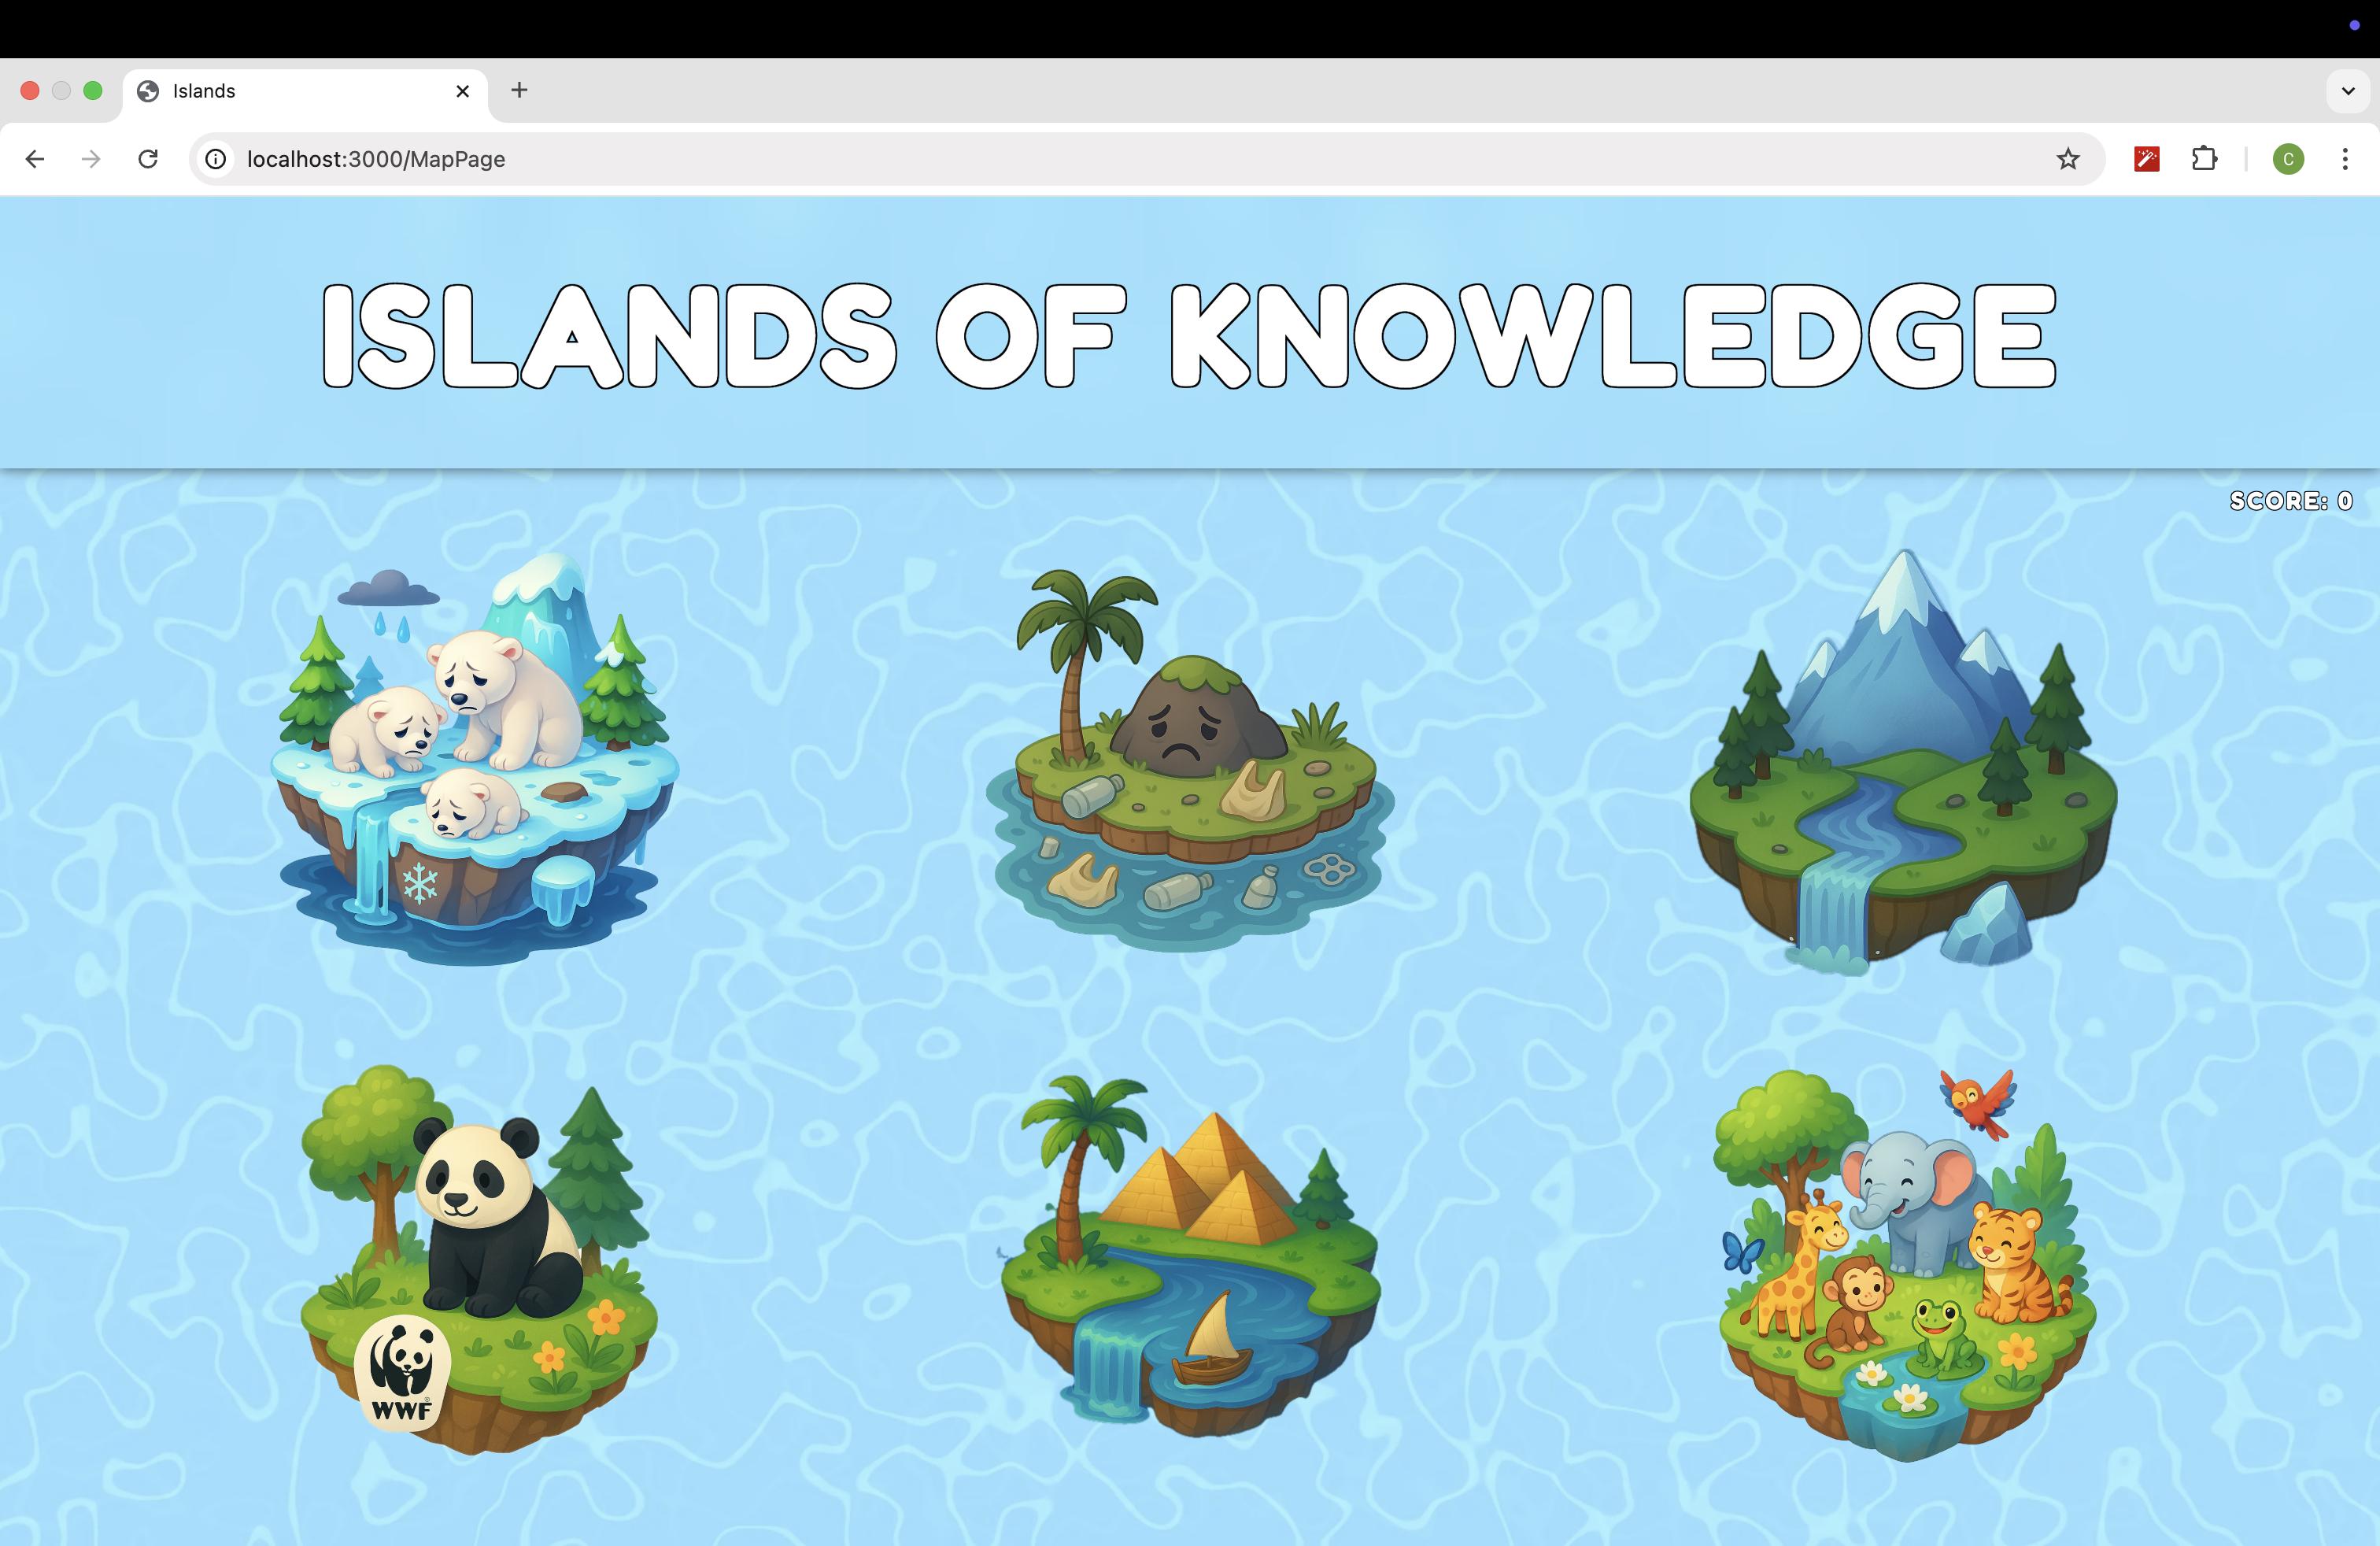
\includegraphics[width=0.9\textwidth]{figures/map.png}
        \caption{Island map with clickable islands.}
        \label{fig:map}
    \end{minipage}%
    \hfill
    \begin{minipage}[b]{0.5\textwidth}
        \centering
        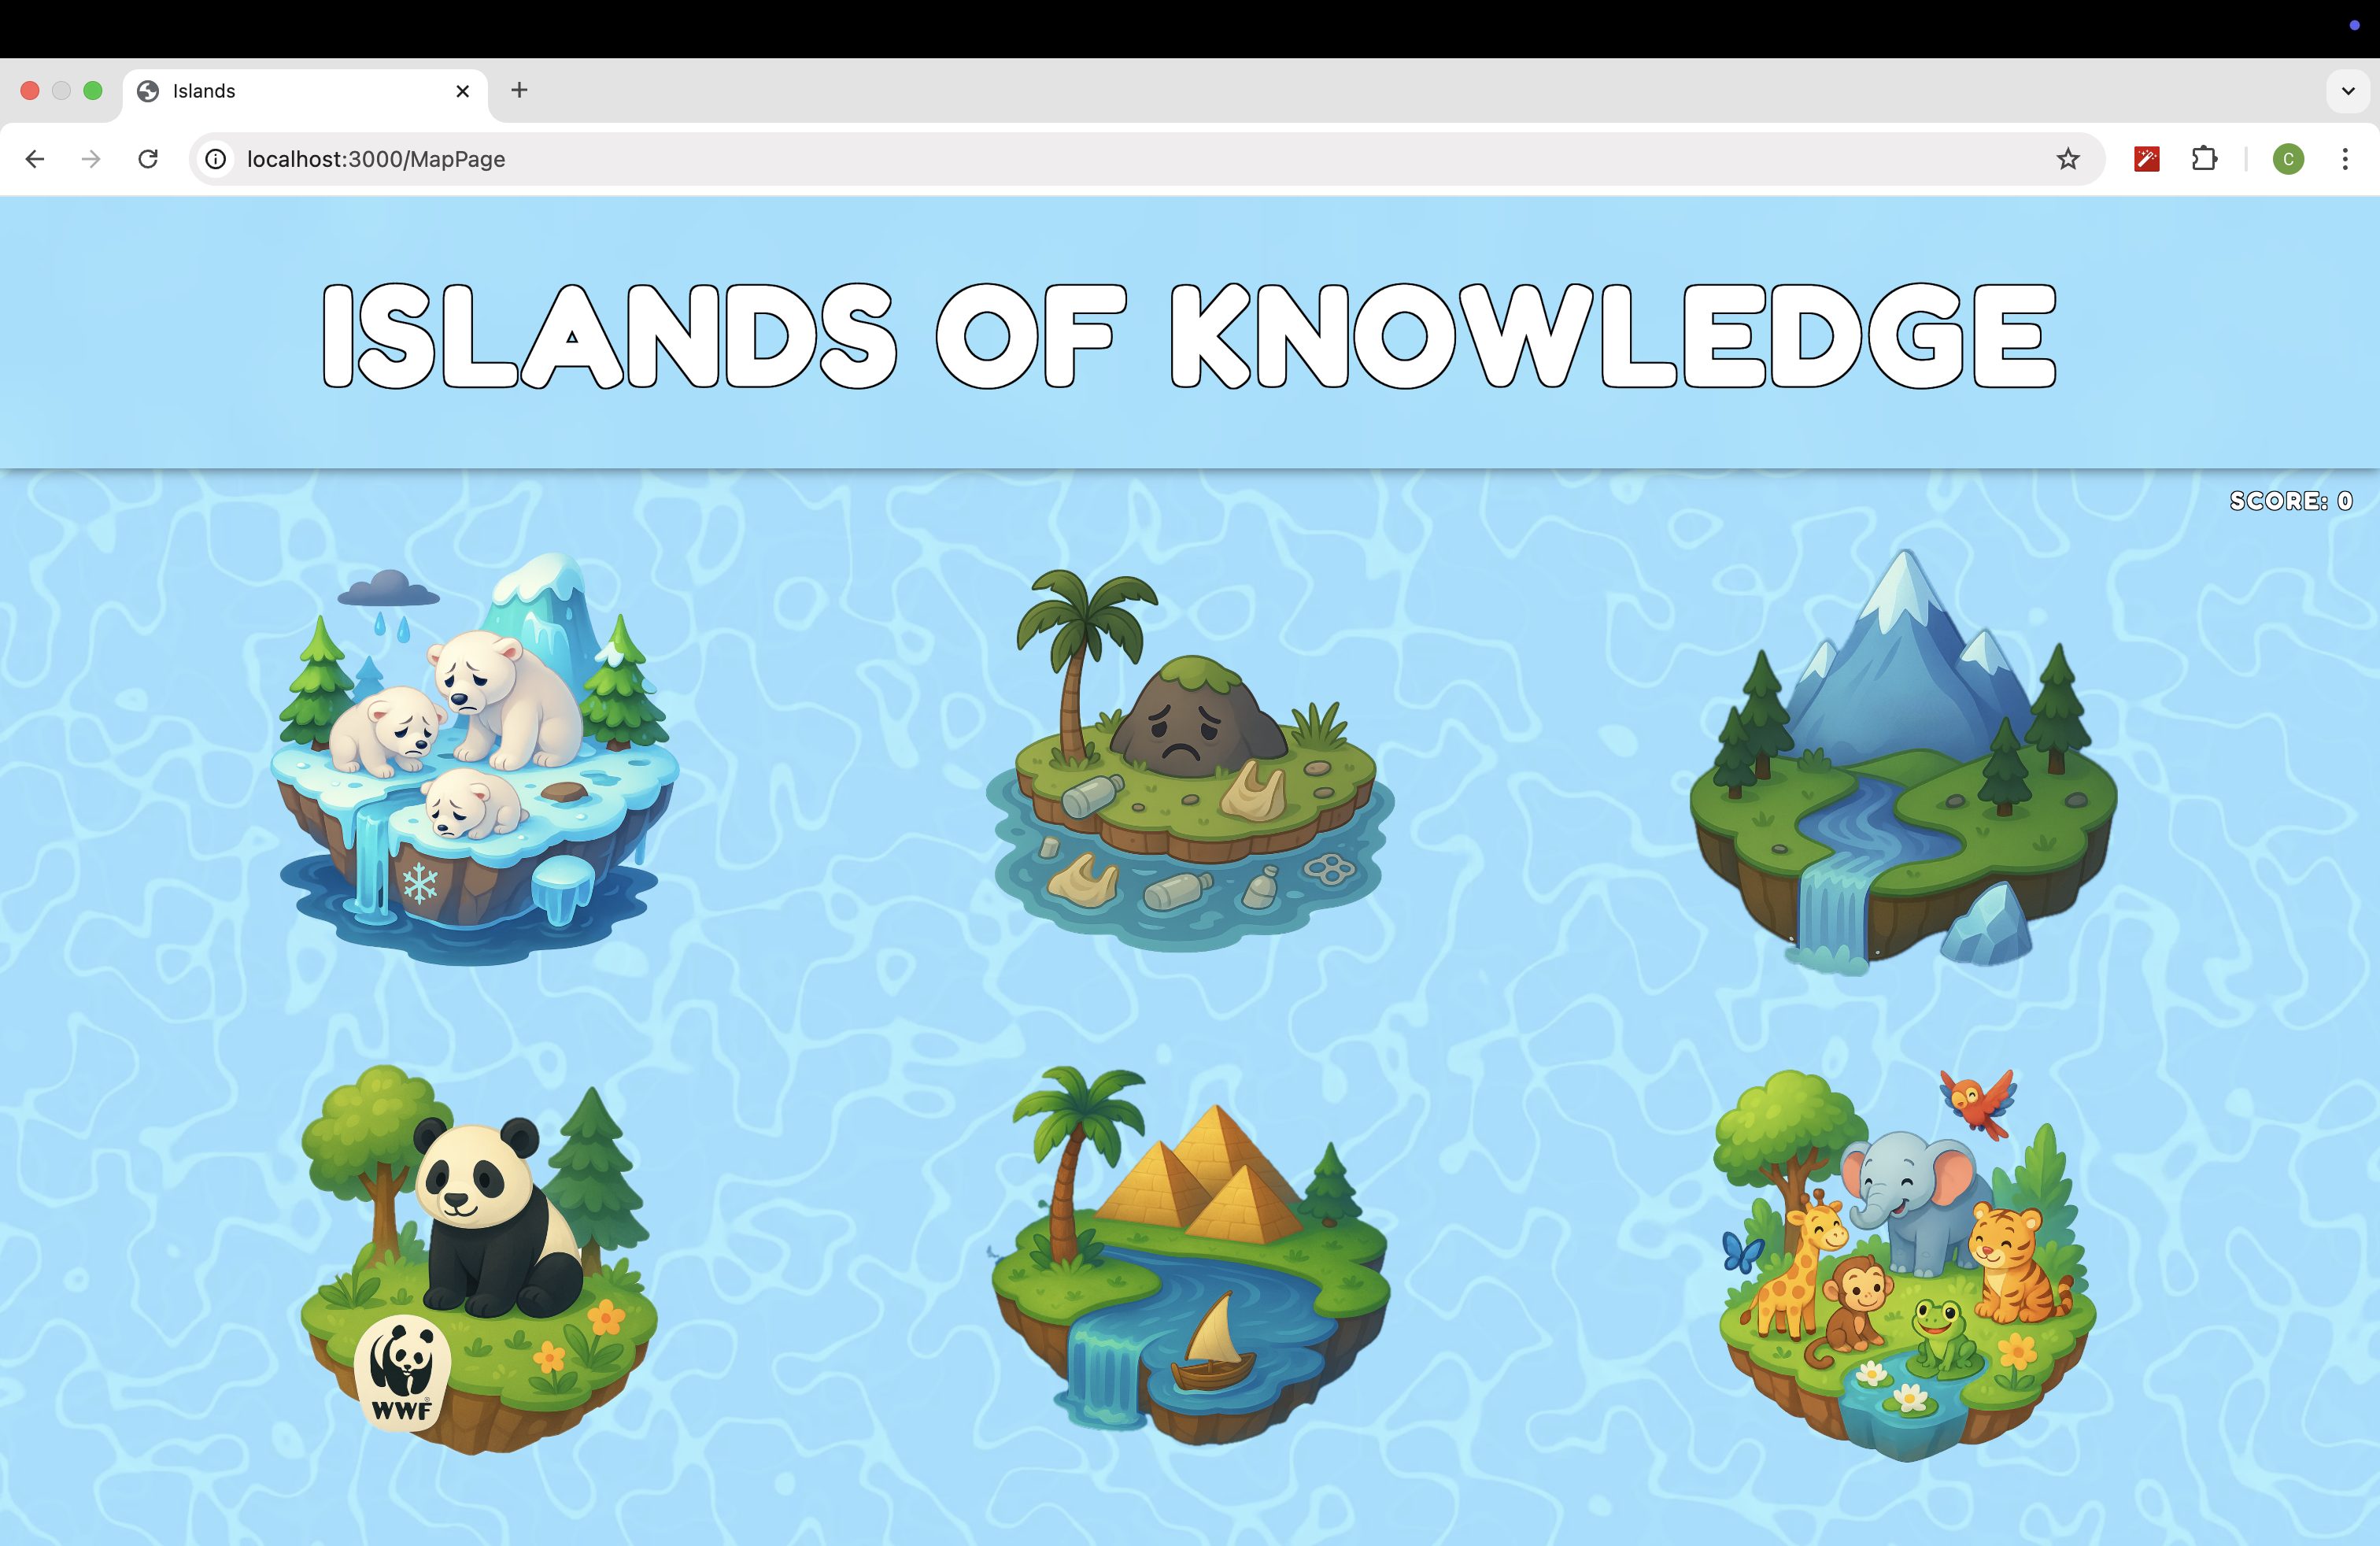
\includegraphics[width=0.9\textwidth]{figures/map-hover.png}
        \caption{Hover effect on islands.}
        \label{fig:map-hover}
    \end{minipage}
\end{figure}

\subsubsection*{\textbf{Step 5: Tool Choice}}

After selecting an island, the child reaches a tool selection page (Fig.~\ref{fig:choice-page}) where they choose between a traditional search engine (Google) and a large language model (Gemini).

\begin{figure}[H]
    \centering
    \includegraphics[width=0.5\textwidth]{figures/choice-page.png}
    \caption{Tool choice screen.}
    \label{fig:choice-page}
\end{figure}

\subsubsection*{\textbf{Step 6: Using Google}}

If the child selects Google, they are presented with a simulated Search Engine landing page (Fig.~\ref{fig:google}). The interface and behavior mimic real-life scenarios (Fig.~\ref{fig:serp}). Clicking on links opens them in a new tab.

\begin{figure}[H]
    \begin{minipage}[b]{0.5\textwidth}
        \centering
        \includegraphics[width=0.9\textwidth]{figures/google.png}
        \caption{Simulated Google landing.}
        \label{fig:google}
    \end{minipage}
    \hfill
    \begin{minipage}[b]{0.5\textwidth}
        \centering
        \includegraphics[width=0.9\textwidth]{figures/serp.png}
        \caption{Google search results with clickable links.}
        \label{fig:serp}
    \end{minipage}%
\end{figure}

\subsubsection*{\textbf{Step 7: Using Gemini}}

Alternatively, children can choose Gemini, where a chat-like interface appears (Fig.~\ref{fig:gemini}). A waiting screen mimics the LLM response delay after sending a prompt (Fig.~\ref{fig:gemini-waiting}), followed by the result output (Fig.~\ref{fig:gemini-results}).

\begin{figure}[H]
    \begin{minipage}[b]{0.5\textwidth}
        \centering
        \includegraphics[width=0.9\textwidth]{figures/gemini.png}
        \caption{Gemini chat interface.}
        \label{fig:gemini}
    \end{minipage}%
    \hfill
    \begin{minipage}[b]{0.5\textwidth}
        \centering
        \includegraphics[width=0.9\textwidth]{figures/gemini-waiting.png}
        \caption{Waiting screen for Gemini response.}
        \label{fig:gemini-waiting}
    \end{minipage}
    \begin{minipage}[b]{0.5\textwidth}
        \centering
        \includegraphics[width=0.9\textwidth]{figures/gemini-results.png}
        \caption{Gemini response output.}
        \label{fig:gemini-results}
    \end{minipage}
\end{figure}

\subsubsection*{\textbf{Step 8: Submitting an Answer}}

After exploring the results, the child can type the final answer (Fig.~\ref{fig:answer}). Once submitted, the user is redirected to the map page, and the island becomes inactive. If the child attempts to revisit a completed island, a warning is shown (Fig.~\ref{fig:warning}).

\begin{figure}[H]
    \begin{minipage}[b]{0.5\textwidth}
        \centering
        \includegraphics[width=0.9\textwidth]{figures/answer.png}
        \caption{Final answer submission screen.}
        \label{fig:answer}
    \end{minipage}%
    \hfill
    \begin{minipage}[b]{0.5\textwidth}
        \centering
        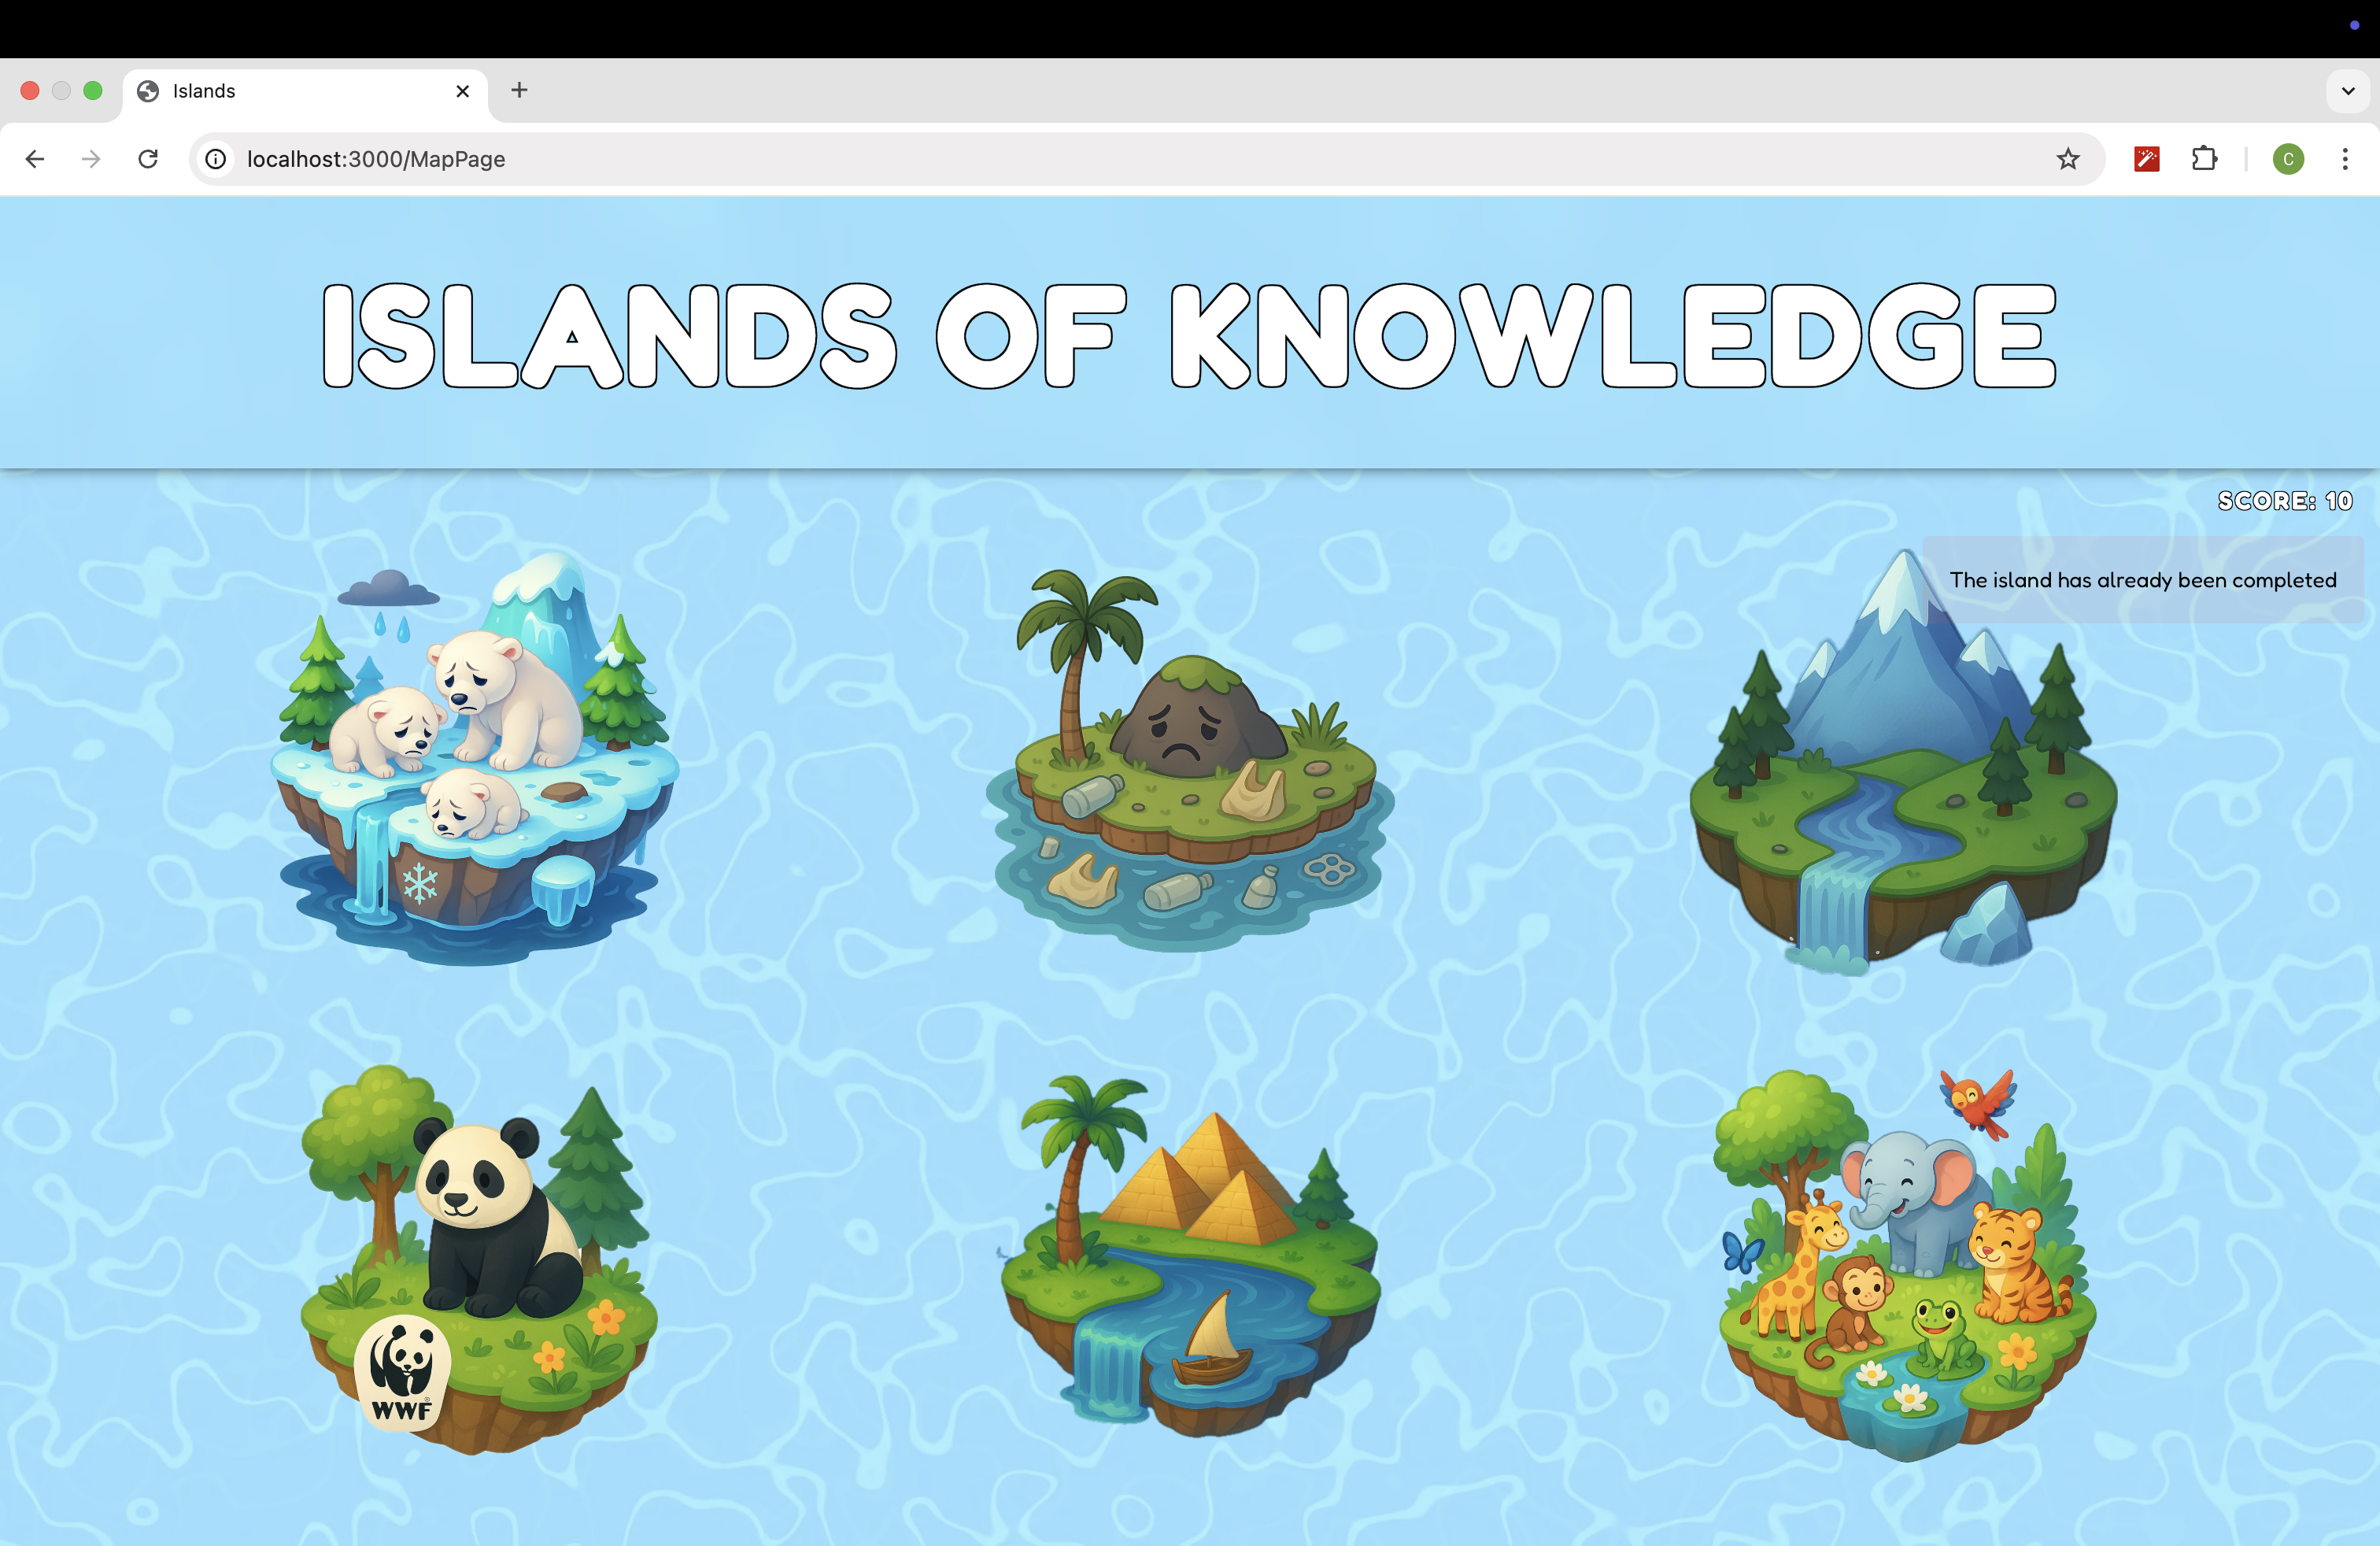
\includegraphics[width=0.9\textwidth]{figures/warning.png}
        \caption{Can't click on a completed island.}
        \label{fig:warning}
    \end{minipage}
\end{figure}

\subsubsection*{\textbf{Step 9: Final Page and Data Export}}

After completion of all six islands, the child sees their final score (Fig.~\ref{fig:final-score}). Each completed island contributes 10 points, with a maximum of 60.

To end the session, a password-protected download prompt is shown (Fig.~\ref{fig:download}), allowing the teacher or researcher to save all session data locally. It was a design choice to use the brower's prompt functionality instead of a custom modal, to discourage children from trying to tamper with the data export.

\begin{figure}[H]
    \begin{minipage}[b]{0.5\textwidth}
        \centering
        \includegraphics[width=0.9\textwidth]{figures/final-score.png}
        \caption{Final score screen after completing all islands.}
        \label{fig:final-score}
    \end{minipage}%
    \hfill
    \begin{minipage}[b]{0.5\textwidth}
        \centering
        \includegraphics[width=0.9\textwidth]{figures/download.png}
        \caption{Password-protected data download prompt.}
        \label{fig:download}
    \end{minipage}
\end{figure}

\subsection{\textbf{Experts' Feedback}}
The tool was presented to two experts, teachers with experience in working with children and technology. They provided valuable feedback on the design and usability of the tool.

HERE COMMENTS FROM TEACHERS

\newpage

%%%%%%%%%%%%%%%%%%%%%%%%%%%% CONCLUSIONS %%%%%%%%%%%%%%%%%%%%%%%%%%%%%

\section{\textbf{Conclusions}}

\subsection{\textbf{Future Work}}

Although the current prototype is functional and is already suitable for small-scale research studies, further improvements can be made in future iterations to improve usability, data collection, and scalability.

\subsubsection*{\textbf{User Interface and Usability Testing}}
The current interface was designed based on the insights of the literature and internal feedback, but because the design interface could have been a whole project on its own, it can be improved. Furthermore, it has not yet been tested with children in real-life settings. One key area for future work is to conduct formal usability testing sessions with children of different age groups. These sessions would help identify which parts of the UI are intuitive, which are appealing, and which are confusing or too complex. For example, visual feedback (for example hover animations, tool choices, iconography) may need to be adjusted based on children’s preferences and cognitive abilities. Additionally, working with experts in child-computer interaction and UX/UI could help refine the design to better suit the target audience.

\subsubsection*{\textbf{Extending Data Collection}}

The current version of the system already collects a wide set of interaction data, including query logs, tool switches, time spent, and submitted responses. However, there is room for improvement and expansion. Future versions could include additional behavioral signals, such as
\begin{itemize}
    \item Mouse movement and hover times to infer hesitation or curiosity.
    \item Scroll depth within the SERP.
    \item Optional feedback prompts for children to self-report satisfaction or perceived difficulty.
\end{itemize}


\subsubsection*{\textbf{Improving Efficiency and Scalability}}

In the current version of the system, all interaction data is stored locally in the browser and must be manually exported at the end of each session. Although this solution is suitable for small-scale studies or pilot experiments, it introduces several limitations when conducting larger studies.

Managing data from multiple devices becomes time-consuming and there is a risk of losing session data if a participant closes the browser before exporting. Relying on browser-based password prompts also provides only minimal protection and may not be ideal in more formal research contexts.

A possible solution could be to integrate a back-end infrastructure that stores the data in a centralized manner, allowing researchers to:
\begin{itemize}
    \item Monitor sessions in real time, even across multiple classrooms or devices.
    \item Automatically collect and aggregate data without manual intervention.
    \item Minimize the risk of data loss due to user error or technical problems.
\end{itemize}







\newpage

%%%%% BIBLIOGRAPHY %%%%%
\bibliographystyle{abbrv}
\bibliography{references}

\end{document}
